\documentclass{beamer}
\usepackage{beamerthemesplit}
\usepackage{wrapfig}
\usetheme{SPbGU}
\usepackage{pdfpages}
\usepackage{amsmath}
\usepackage{cmap} 
\usepackage[T2A]{fontenc} 
\usepackage[utf8]{inputenc}
\usepackage[english,russian]{babel}
\usepackage{indentfirst}
\usepackage{amsmath}
\usepackage{tikz}
\usepackage{multirow}
\usepackage[noend]{algpseudocode}
\usepackage{algorithm}
\usepackage{algorithmicx}
\usepackage{epstopdf}
\usetikzlibrary{shapes,arrows}
\usepackage{fancyvrb}
\newtheorem{rutheorem}{Theorem}
\beamertemplatenavigationsymbolsempty

\title[]{Relaxed Parsing of Regular Approximations of String-Embedded Languages}
\institute[SPbSU]{
Saint Petersburg State University \\
JetBrains Programming Languages and Tools Lab }

\author[Ekaterina Verbitskaia]{Ekaterina Verbitskaia}

\date{26/08/2015}

\definecolor{orange}{RGB}{179,36,31}

\begin{document}
{

\begin{frame}
  \begin{center}
  {
\includegraphics[width=1cm]{SPbGU_Logo.png}}
  \end{center}
  \titlepage
\end{frame}
}

\begin{frame}[fragile]
  \transwipe[direction=90]
  \frametitle{String-embedded code}
  \begin{itemize}
    \item Embedded SQL
      \begin{Verbatim}[commandchars=\\\{\}]
\textcolor{blue}{SqlCommand} myCommand = new \textcolor{blue}{SqlCommand}(
    \textcolor{orange}{"SELECT * FROM table WHERE Column = @Param2"},
    myConnection);
myCommand.Parameters.Add(myParam2);
      \end{Verbatim}

    \item Dynamic SQL
      \begin{Verbatim}[commandchars=\\\{\}]
\textcolor{blue}{IF} @X = @Y
    \textcolor{blue}{SET} @TBL = \textcolor{orange}{' #table1 '}
\textcolor{blue}{ELSE}
    \textcolor{blue}{SET} @TBL = \textcolor{orange}{' table2 '}
\textcolor{blue}{SET} @S = \textcolor{orange}{'SELECT x FROM'} + @TBL + \textcolor{orange}{'WHERE ISNULL(n,0) > 1'}
EXECUTE (@S)
       \end{Verbatim}
    \end{itemize}
\end{frame}

\begin{frame}
  \transwipe[direction=90]
  \frametitle{Problems}  
  \begin{itemize}
    \item String-embedded code are expressions in some programming language
    \begin{itemize}
      \item It may be necessary to support them in IDE: code highlighting, 
autocomplete, refactorings
      \item It may be necessary to transform them: migration of legacy software 
to new platforms
      \item It may be necessary to detect vulnerabilities in such code
      \item Any other problems of programming languages can occur
    \end{itemize}
  \end{itemize}
\end{frame}

\begin{frame}
  \transwipe[direction=90]
  \frametitle{Static analysis of string-embedded code}  
  \begin{itemize}
    \item Performed without programm execution
    \item Checks that the set of properties holds for each possible expression value
  \end{itemize}
  
  \begin{itemize}
    \item Undecidable for string-embedded code in the general case
    \item The set of possible expression values is over approximated and then 
the approximation is analysed
  \end{itemize}
\end{frame}

\begin{frame}
  \transwipe[direction=90]
  \frametitle{Existing tools}
  \begin{itemize}
    \item PHP String Analyzer, Java String Analyzer, Alvor
    \begin{itemize}
      \item Static analyzers for PHP, Java, and SQL embedded into Java 
respectively
    \end{itemize}

    \item Kyung-Goo Doh et al.
    \begin{itemize}
      \item Checks syntactical correctness of embedded code
    \end{itemize}

    \item PHPStorm
    \begin{itemize}
      \item IDE for PHP with support of HTML, CSS, JavaScript
    \end{itemize}

    \item IntelliLang
    \begin{itemize}
      \item PHPStorm and IDEA plugin, supports various languages    
    \end{itemize} 

    \item STRANGER
    \begin{itemize}
      \item Vulnerability detection of PHP
    \end{itemize}
  \end{itemize}
  
  \begin{itemize}
    \item Flaws
    \begin{itemize}
      \item Limited functionality
      \item Hard to extend them with new features or support new languages
      \item Do not create structural representation of code
    \end{itemize}
  \end{itemize}
\end{frame}


\begin{frame}
  \transwipe[direction=90]
  \frametitle{Static analysis of string-embedded code: the scheme}
  \begin{itemize}
    \item Identification of hotspots: points of interest, where the analysis is 
desirable
    \item Approximation construction
    \item Lexical analysis
    \item \textbf{Syntactic analysis}
    \item Semantic analysis
  \end{itemize}
\end{frame}



\begin{frame}[fragile]
\transwipe[direction=90]
\frametitle{Static analysis of string-embedded code: the scheme}

\begin{tabular}{p{4.5cm} p{8cm}}
Code: hotspot is marked
&
\begin{minipage}[t]{5cm}

\begin{Verbatim}[commandchars=\\\{\}]
\textcolor{blue}{string} res = \textcolor{orange}{""};
\textcolor{blue}{for}(i = 0; i < l; i++)
    res = \textcolor{orange}{"()"} + res;
\fbox{\textcolor{blue}{use}(res);}

\end{Verbatim}
\end{minipage}

\\ 
Possible values
&
\begin{minipage}[t]{2.5cm}
\begin{Verbatim}[commandchars=\\\{\}]
\{\textcolor{orange}{""}, \textcolor{orange}{"()"},  \textcolor{orange}{"()()"}, ..., \textcolor{orange}{"()"}^l\}
\end{Verbatim}
\end{minipage}

\\
Regular approximation
&
\begin{minipage}[t]{4cm}
  \begin{Verbatim}[commandchars=\\\{\}]
(\textcolor{orange}{"()"})*
  \end{Verbatim} 
\end{minipage}

\\
Approximation
&
\begin{minipage}[t]{3cm}
\raisebox{-\height}{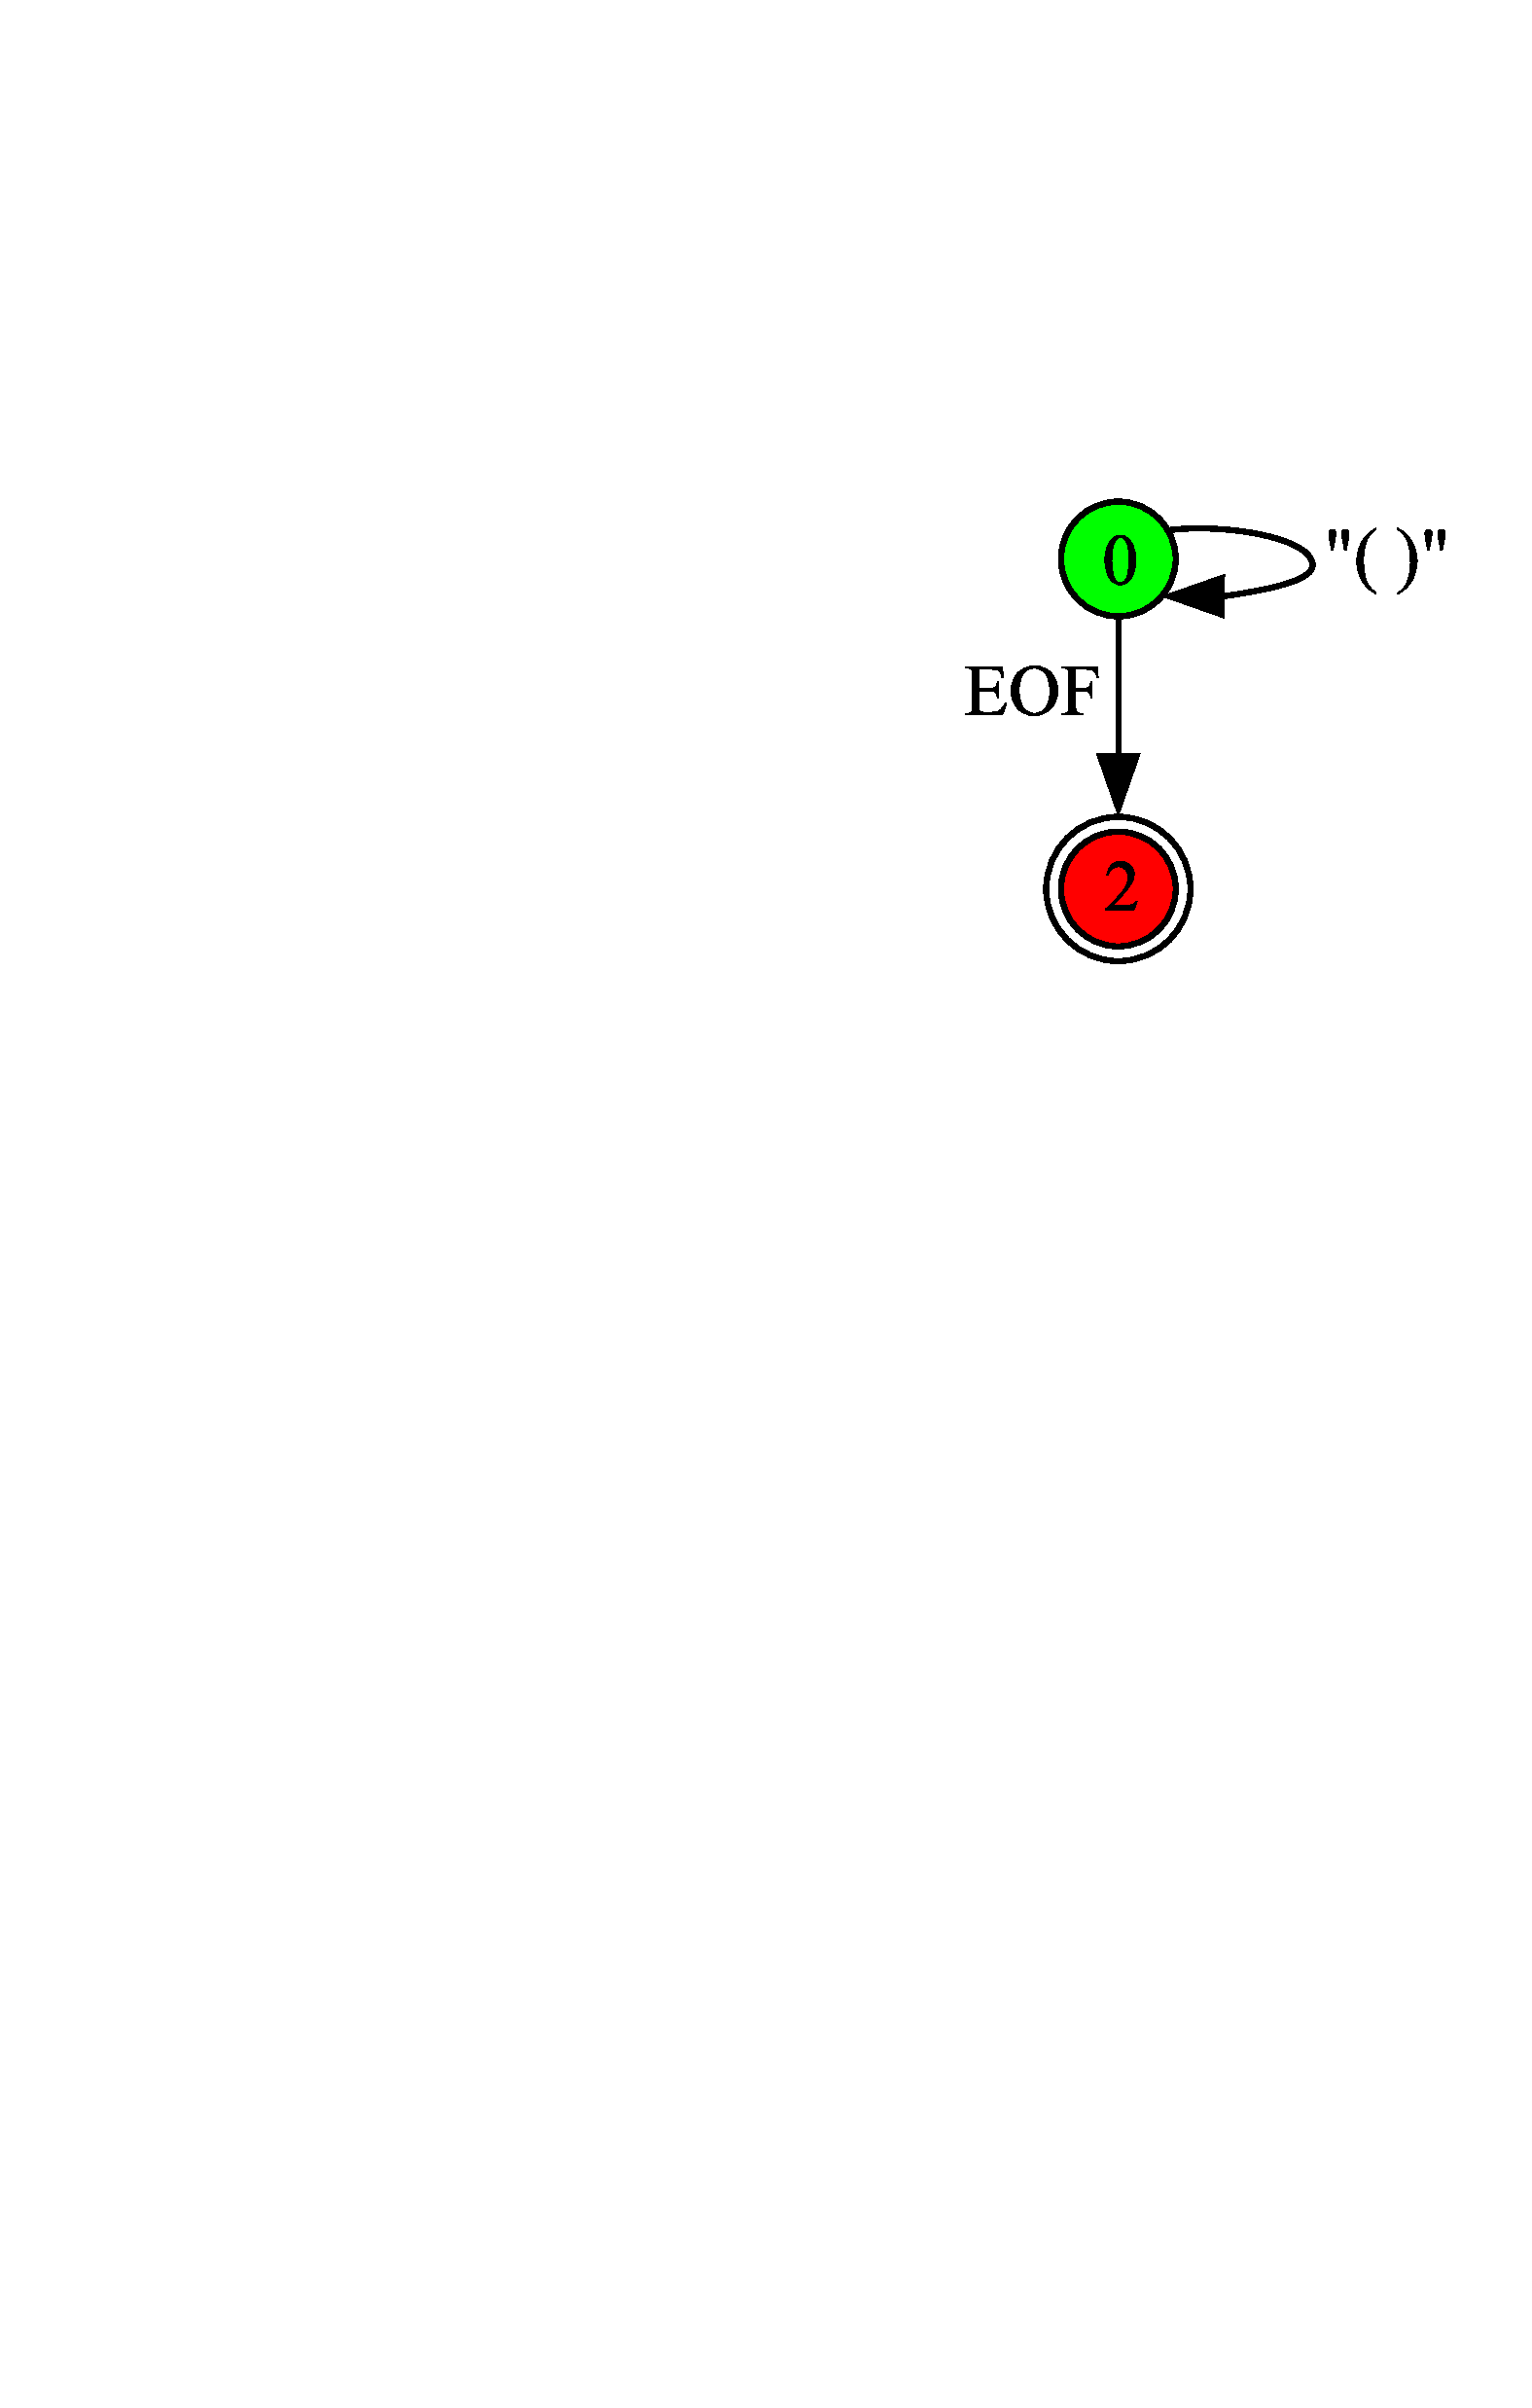
\includegraphics[width=2cm]{pictures/lex1}}
\end{minipage}


\end{tabular}


\end{frame}


\begin{frame}[fragile]
\transwipe[direction=90]
\frametitle{Static analysis of string-embedded code: the scheme}

\begin{tabular}{p{4.5cm} p{8cm}}
\begin{minipage}[t]{4cm}
Approximation\\
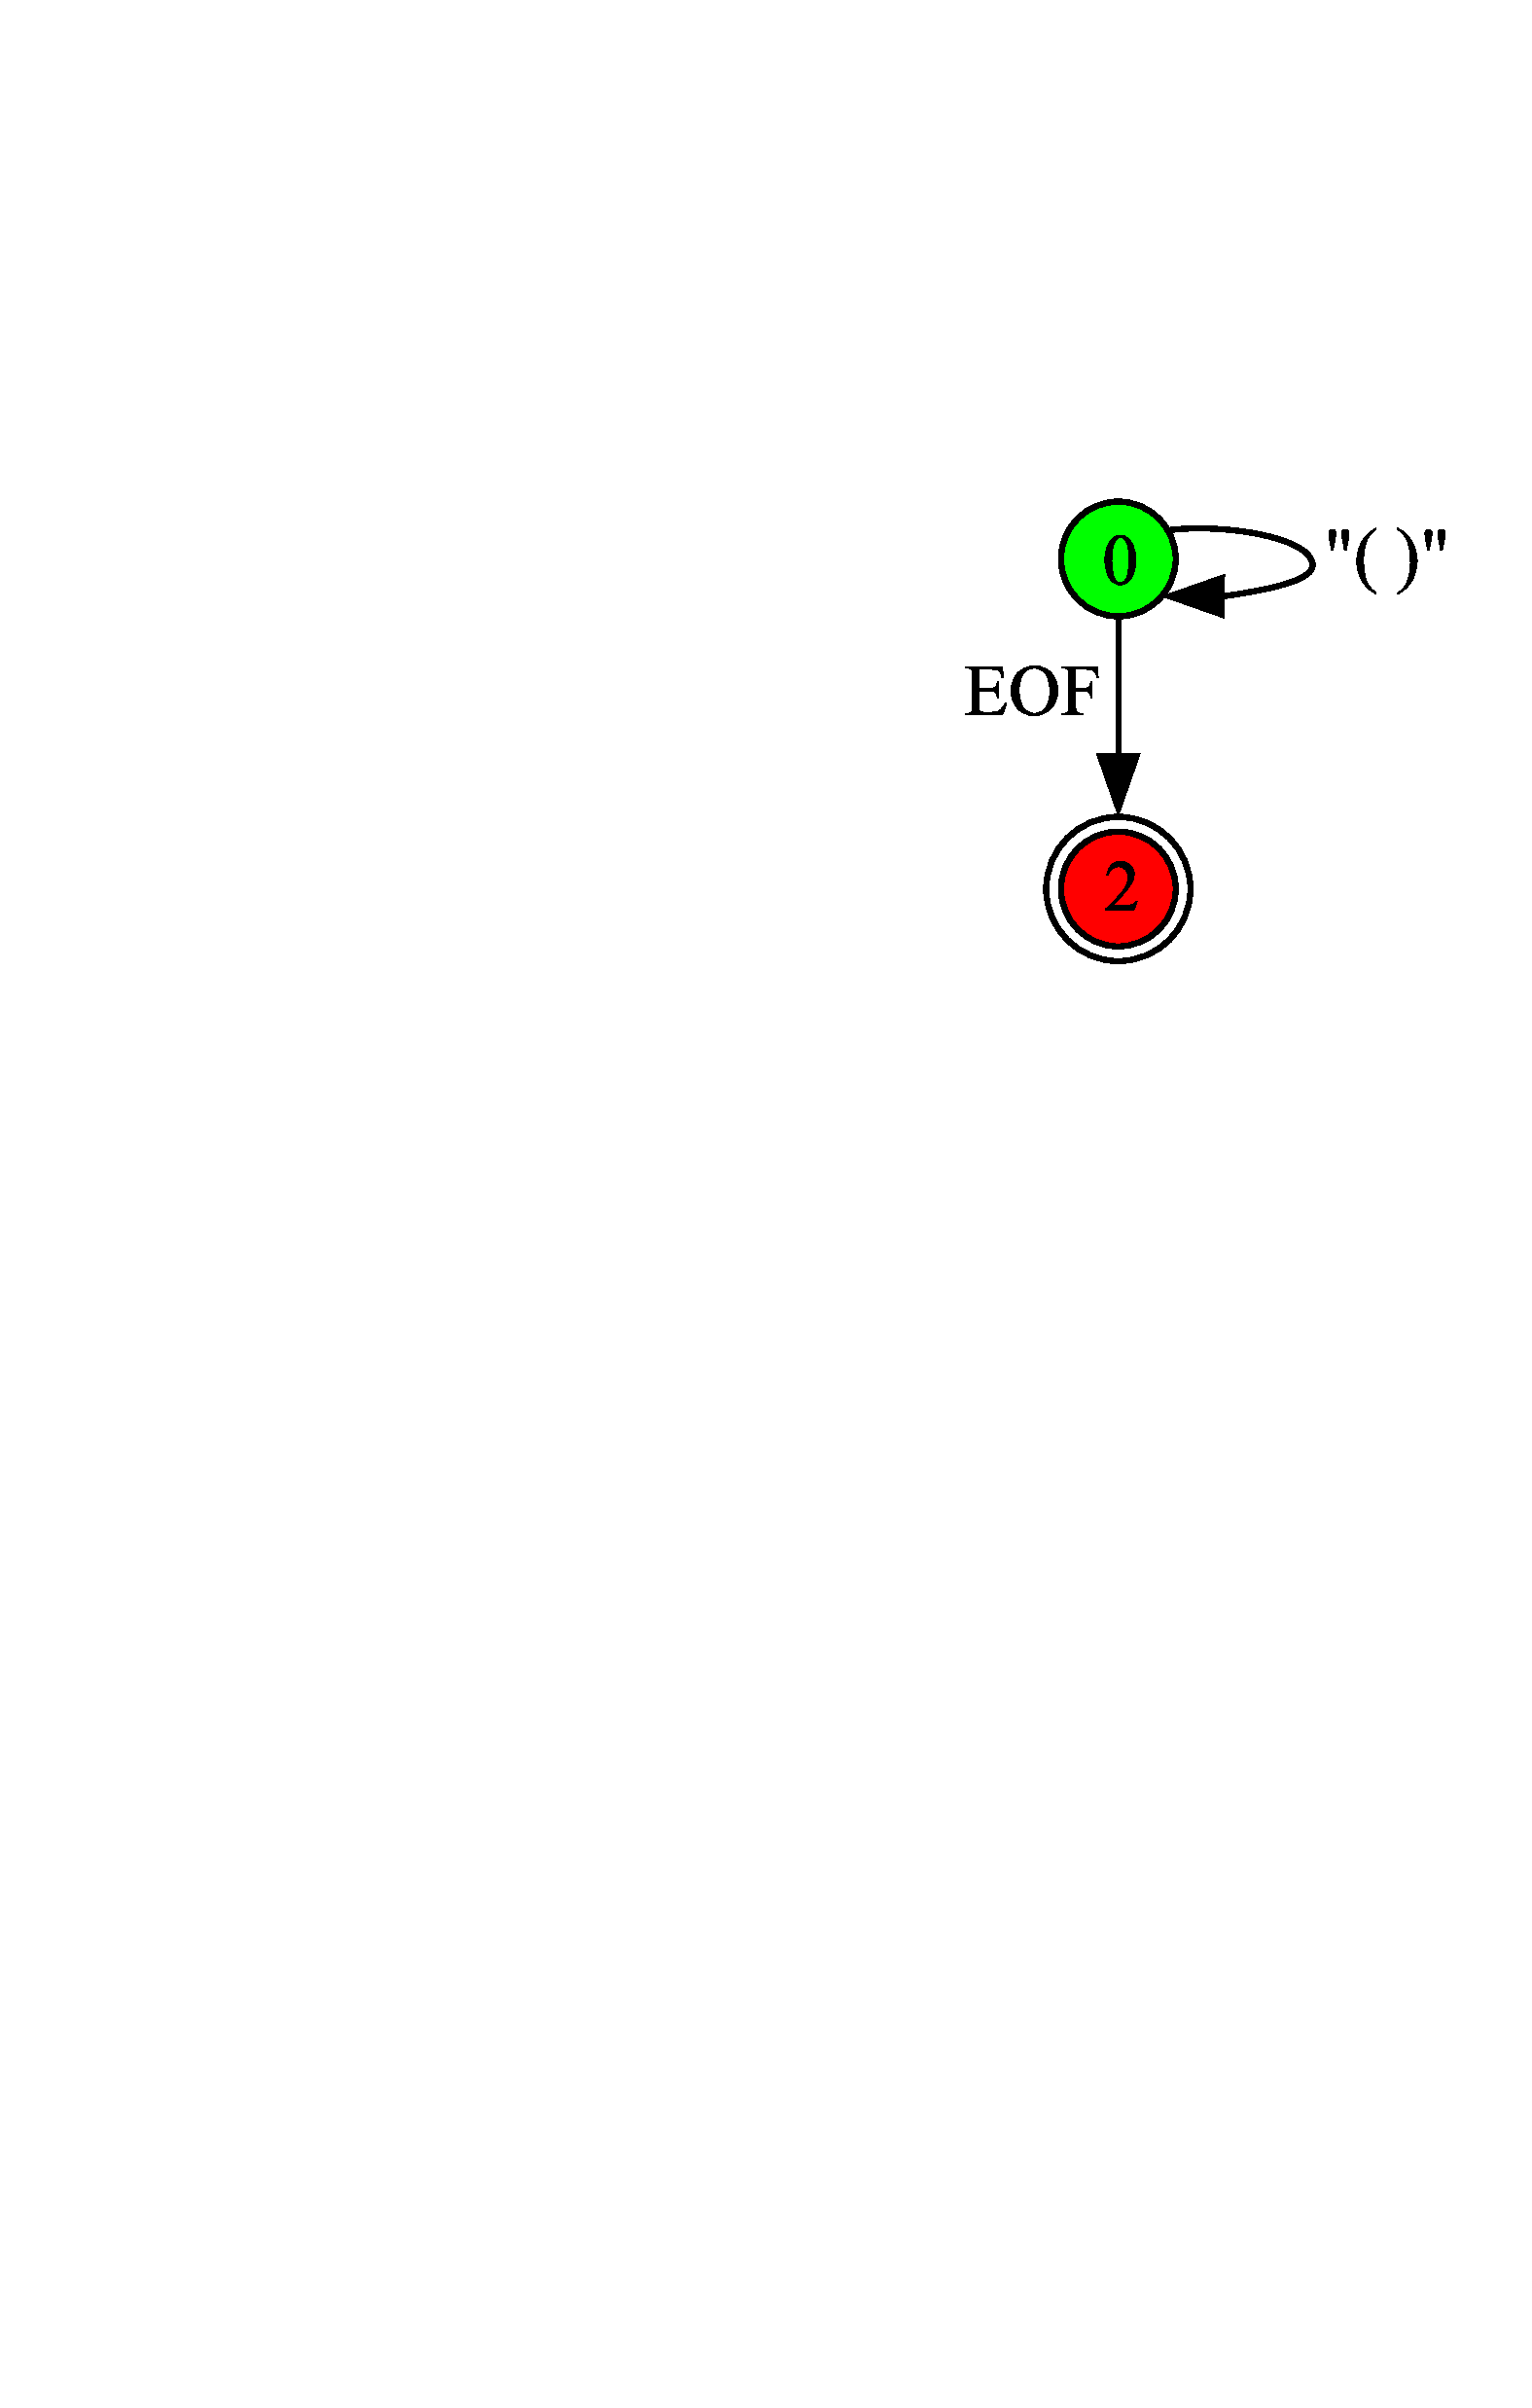
\includegraphics[width=2cm]{pictures/lex1}

After lexing\\
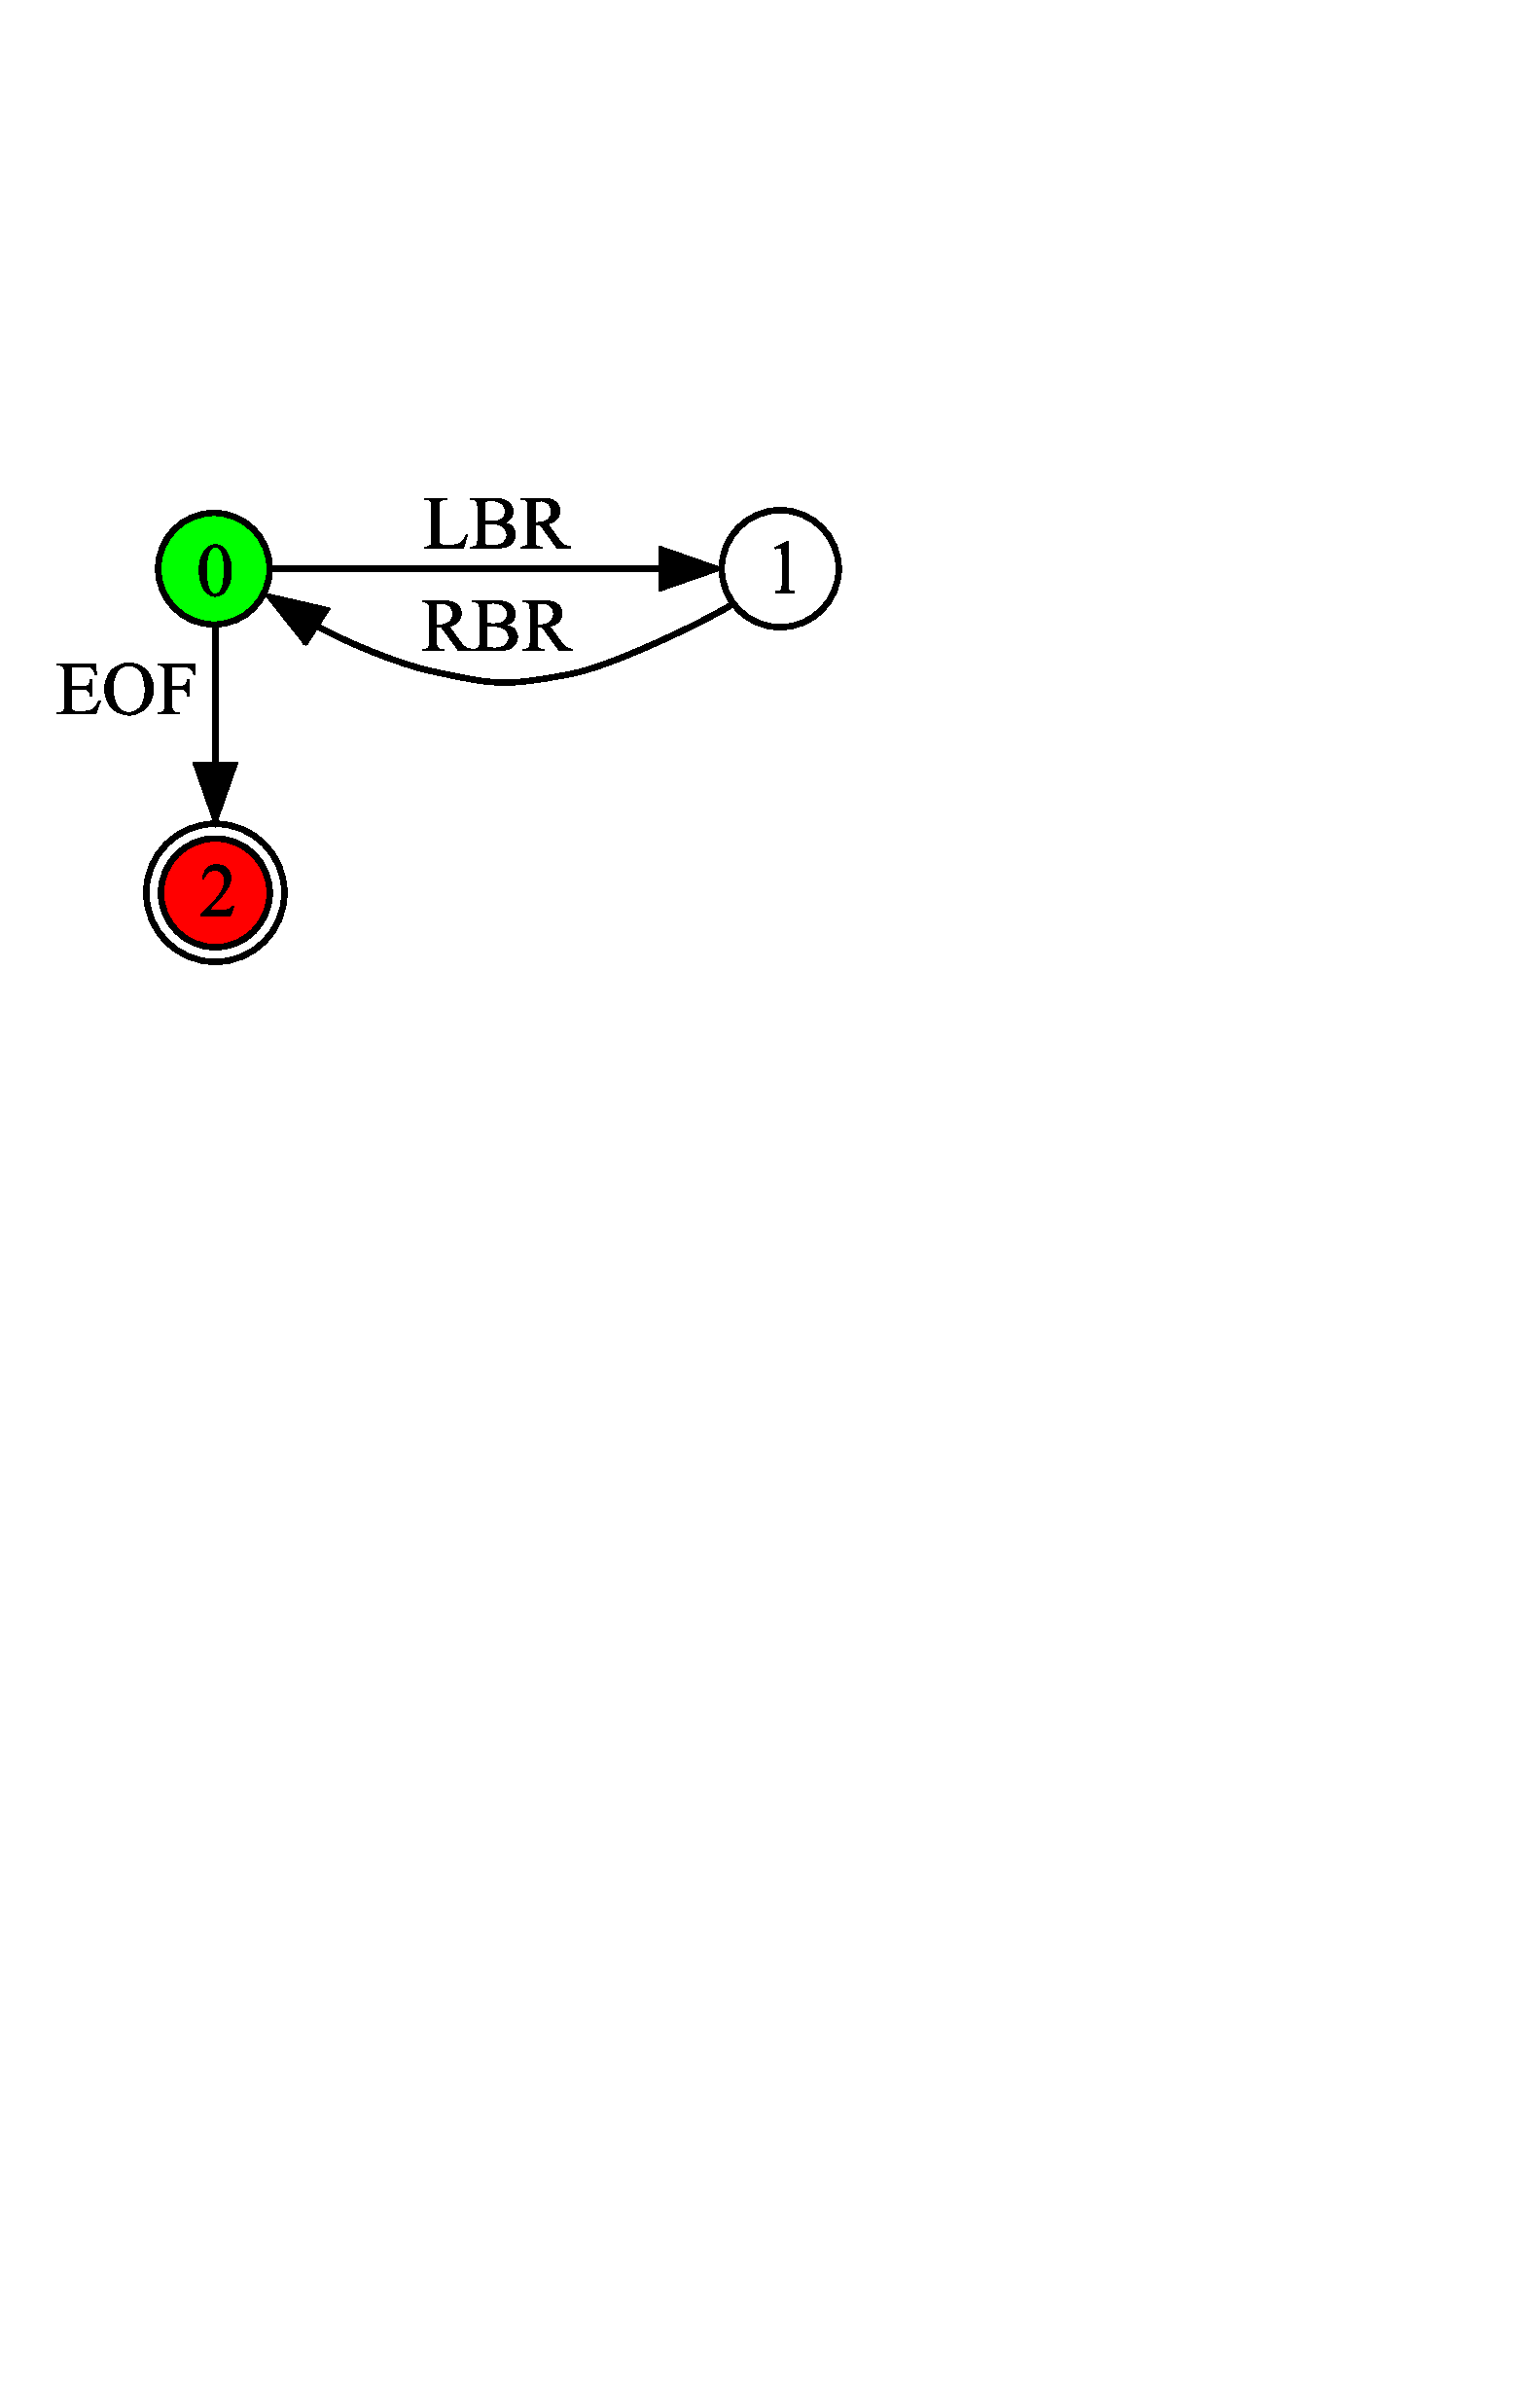
\includegraphics[width=3cm]{pictures/in31}

Grammar\\
\vspace{-5pt}
$$
\begin{array}{crcl}
&start &::=& s \\
&s & ::= & \mbox{\texttt{LBR }} s \mbox{\texttt{ RBR }} s\\
&s & ::= &\epsilon
\end{array}
$$
\end{minipage}
&

\begin{minipage}[t]{8cm}
Parse forest\\
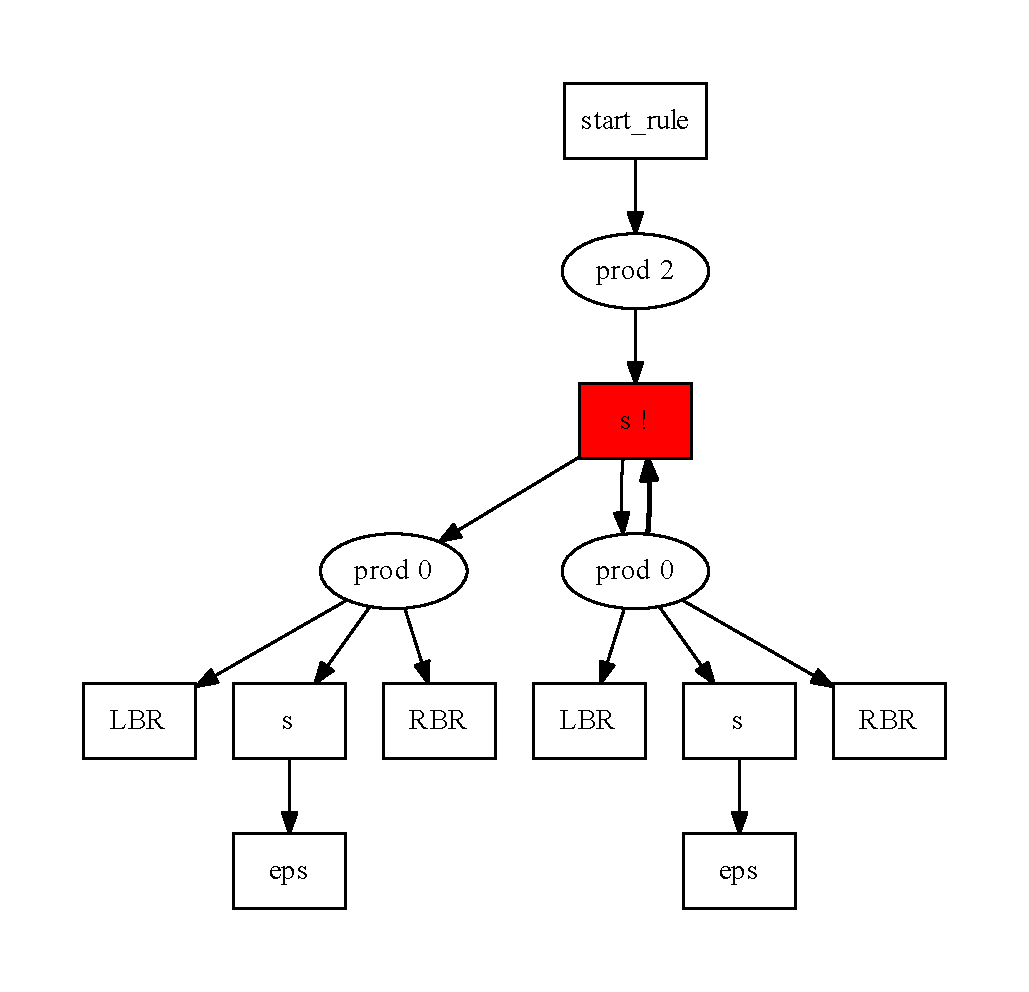
\includegraphics[width=7cm]{pictures/out3}
\end{minipage}

\end{tabular}

\end{frame}

\begin{frame}
  \transwipe[direction=90]
  \frametitle{Problem statement}
  \textbf{The aim} is to develop the algorithm suitable for syntactic analysis of string-embedded code  
  
  \textbf{Tasks}:
  \begin{itemize}
    \item Develop an algorithm for parsing of regular approximation of embedded 
code which produce a finite parse forest
    \item Parse forest should contain a parse tree for every correct (w.r.t. 
reference grammar) string accepted by the input automaton
    \item Incorrect strings should be omitted: no error detection
    \item An algorithm should not depend on the language of the host program 
and the language of embedded code
  \end{itemize}
\end{frame}
            
\begin{frame}
  \transwipe[direction=90]
  \frametitle{Algorithm}
  \begin{itemize}
    \item \textbf{Input}: reference DCF grammar $G$ and DFA graph with no 
$\epsilon$-transitions over the alphabeth of terminals of $G$
    \item \textbf{Output}: finite representation of the trees corresponding to 
all correct string accepted by input automaton
  \end{itemize}
\end{frame}

\begin{frame}
  \transwipe[direction=90]
  \frametitle{Right-Nulled Generalized LR algorithm}
  \begin{itemize}
    \item RNGLR processes context free grammars
    \item In case when LR conflicts occur, parses in each possible way
    \begin{itemize}
      \item Shift/Reduce conflict
      \item Reduce/Reduce conflict
    \end{itemize}
    \item Uses data structures which reduce memory consumption and guarantee 
appropriate time of analysis
  \end{itemize}
\end{frame}

\begin{frame}
  \transwipe[direction=90]
  \frametitle{RNGLR data structures: Graph-Structured Stack}
  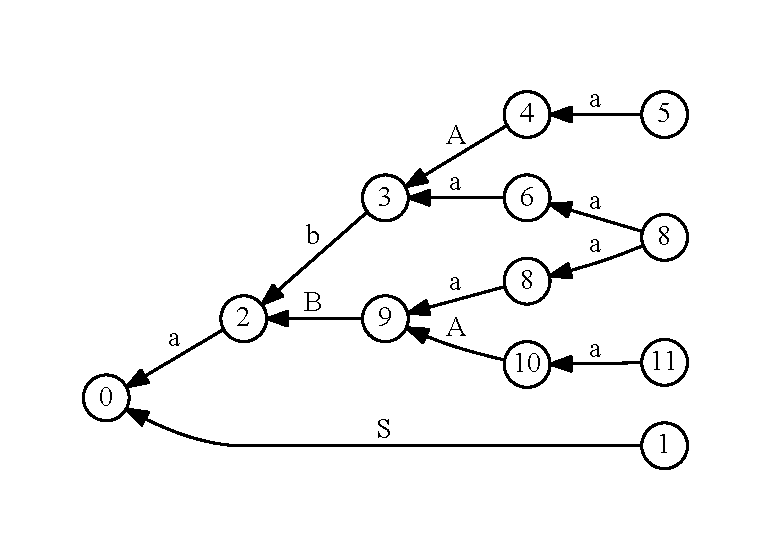
\includegraphics[width=12cm]{pictures/gss_rnglr}
\end{frame}

\begin{frame}
  \transwipe[direction=90]
  \frametitle{RNGLR operations: shift}
  \begin{center}
  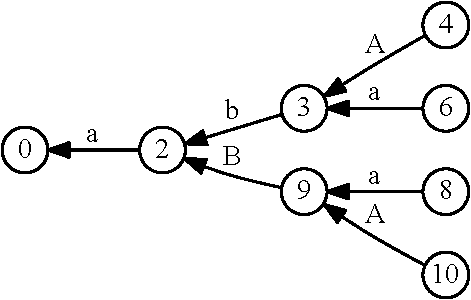
\includegraphics[width=6cm]{pictures/gss_rnglr_shift_1} \\ \vspace{10pt} 
  \pause
  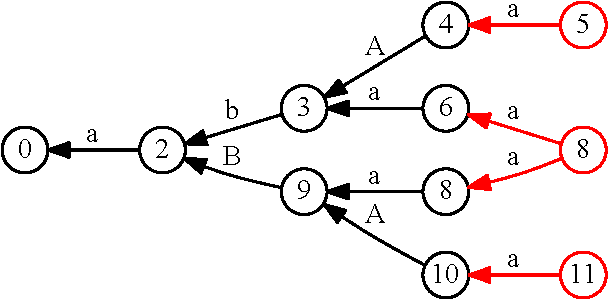
\includegraphics[width=6cm]{pictures/gss_rnglr_shift_2}
  \end{center}
\end{frame}

\begin{frame}
  \transwipe[direction=90]
  \frametitle{RNGLR operations: reduce}
  \begin{center}
  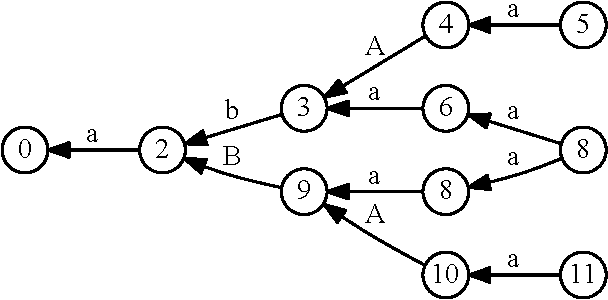
\includegraphics[width=6cm]{pictures/gss_rnglr_reduce_1} \\  \vspace{10pt}
  \pause
  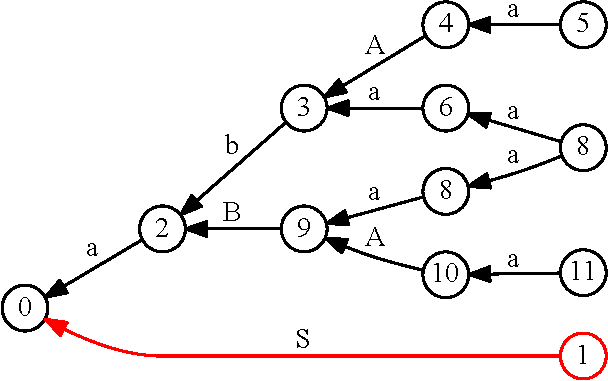
\includegraphics[width=6cm]{pictures/gss_rnglr_reduce_2}
  \end{center}
\end{frame}

\begin{frame}
  \transwipe[direction=90]
  \frametitle{RNGLR}
  \begin{itemize}
    \item Read the input sequentially
  \end{itemize}
  \begin{itemize}
    \item Process all reductions
    \item Shift the next token
  \end{itemize}
  \begin{itemize}
    \item Each time new vertex is added to the GSS, shift is calculated
    \item Each time new edge is created in the GSS, reductions are calculated
  \end{itemize}
\end{frame}



\begin{frame}
  \transwipe[direction=90]
  \frametitle{Algorithm}
  \begin{itemize}
    \item Traverse the automaton graph and sequentially construct GSS, similarly as in RNGLR
    \item New type of ``conflict'': Shift/Shift
  \end{itemize}
  \begin{itemize}
    \item The set of LR-states is associated with each vertex of input graph
    \item The order in which the vertices of input graph are traversed is 
controled with a queue. Whenever new edge is added to GSS, its tail vertex is enqueued
  \end{itemize}
  \begin{itemize}
    \item The algorithm implements relaxed parsing: errors are not detected, 
erroneous strings are ignored
  \end{itemize}
\end{frame}

\begin{frame}
  \transwipe[direction=90]
  \frametitle{Cycles processing: initial stack}
  \begin{center}                                
  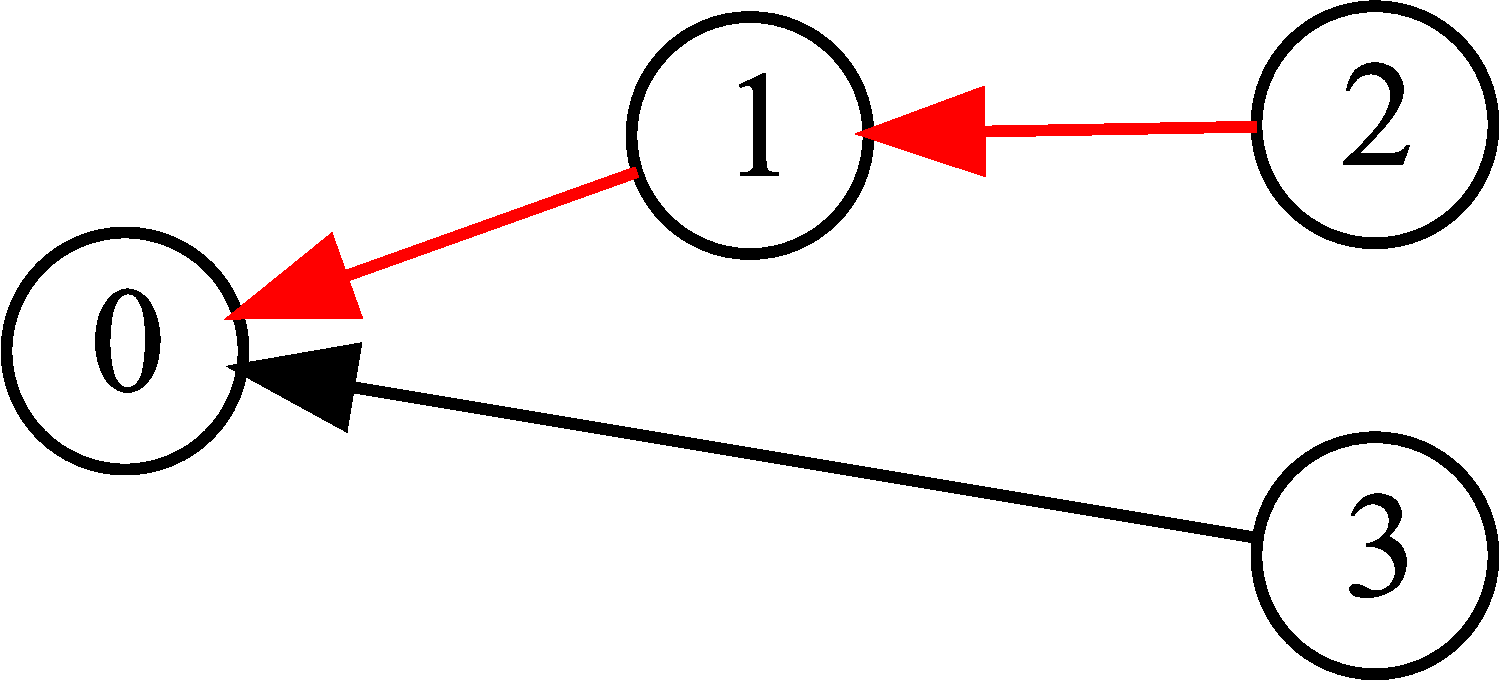
\includegraphics[width=6cm]{pictures/gss_cycle/gss_cycle_init_highlight}
  \end{center}
\end{frame}

\begin{frame}
  \transwipe[direction=90]
  \frametitle{Cycles processing: some edges were added}
  \begin{center}                                
  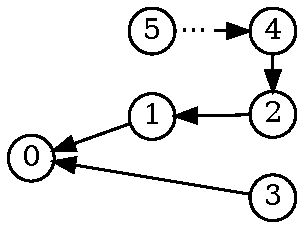
\includegraphics[width=6cm]{pictures/gss_cycle/gss_cycle_no_square}
  \end{center}
\end{frame}

\begin{frame}
  \transwipe[direction=90]
  \frametitle{Cycles processing: cycle closed}
  \begin{center}                                
  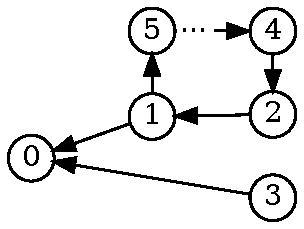
\includegraphics[width=6cm]{pictures/gss_cycle/gss_cycle_no_red_no_highlight}
  \end{center}
\end{frame}

\begin{frame}
  \transwipe[direction=90]
  \frametitle{Cycles processing: new reduction}
  \begin{center}                                
  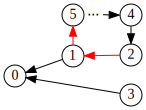
\includegraphics[width=6cm]{pictures/gss_cycle/gss_cycle_no_red}
  \end{center}
\end{frame}

\begin{frame}
  \transwipe[direction=90]
  \frametitle{Cycles processing: new reduction added}
  \begin{center}                                
  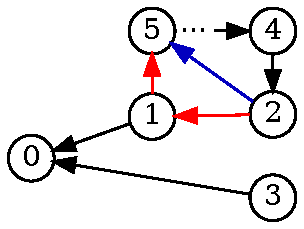
\includegraphics[width=6cm]{pictures/gss_cycle/gss_cycle}
  \end{center}
\end{frame}

\begin{frame}
  \transwipe[direction=90]
  \frametitle{Parse forest construction}
  \begin{itemize}
    \item Shared Packed Parse Forest --- graph, in which all derivation trees are merged
    \item Constructed in the same manner as in the RNGLR-algorithm
    \end{itemize}
    \begin{itemize}
      \item Fragments of derivation trees are associated with GSS edges
      \item Each time shift is processed, new tree of one terminal is created
      \item Each time reduction is processed, new tree with children accumulated along the paths is created
      \begin{itemize}
        \item Children are not copied, they are reused        
      \end{itemize}
      \item The root of resulting tree is associated with GSS edge, corresponding to reduction to the starting nonterminal
      \begin{itemize}
        \item Unreachable vertices are deleted from resulting graph
      \end{itemize}
    \end{itemize}

\end{frame}

\begin{frame}
\transwipe[direction=90]
\frametitle{Algorithm: correctness}
\begin{tabular}{p{5.3cm} p{6.7cm}}
\emph{Correct tree} --- derivation tree of some string accumulated along the 
path in the input graph
&
\\
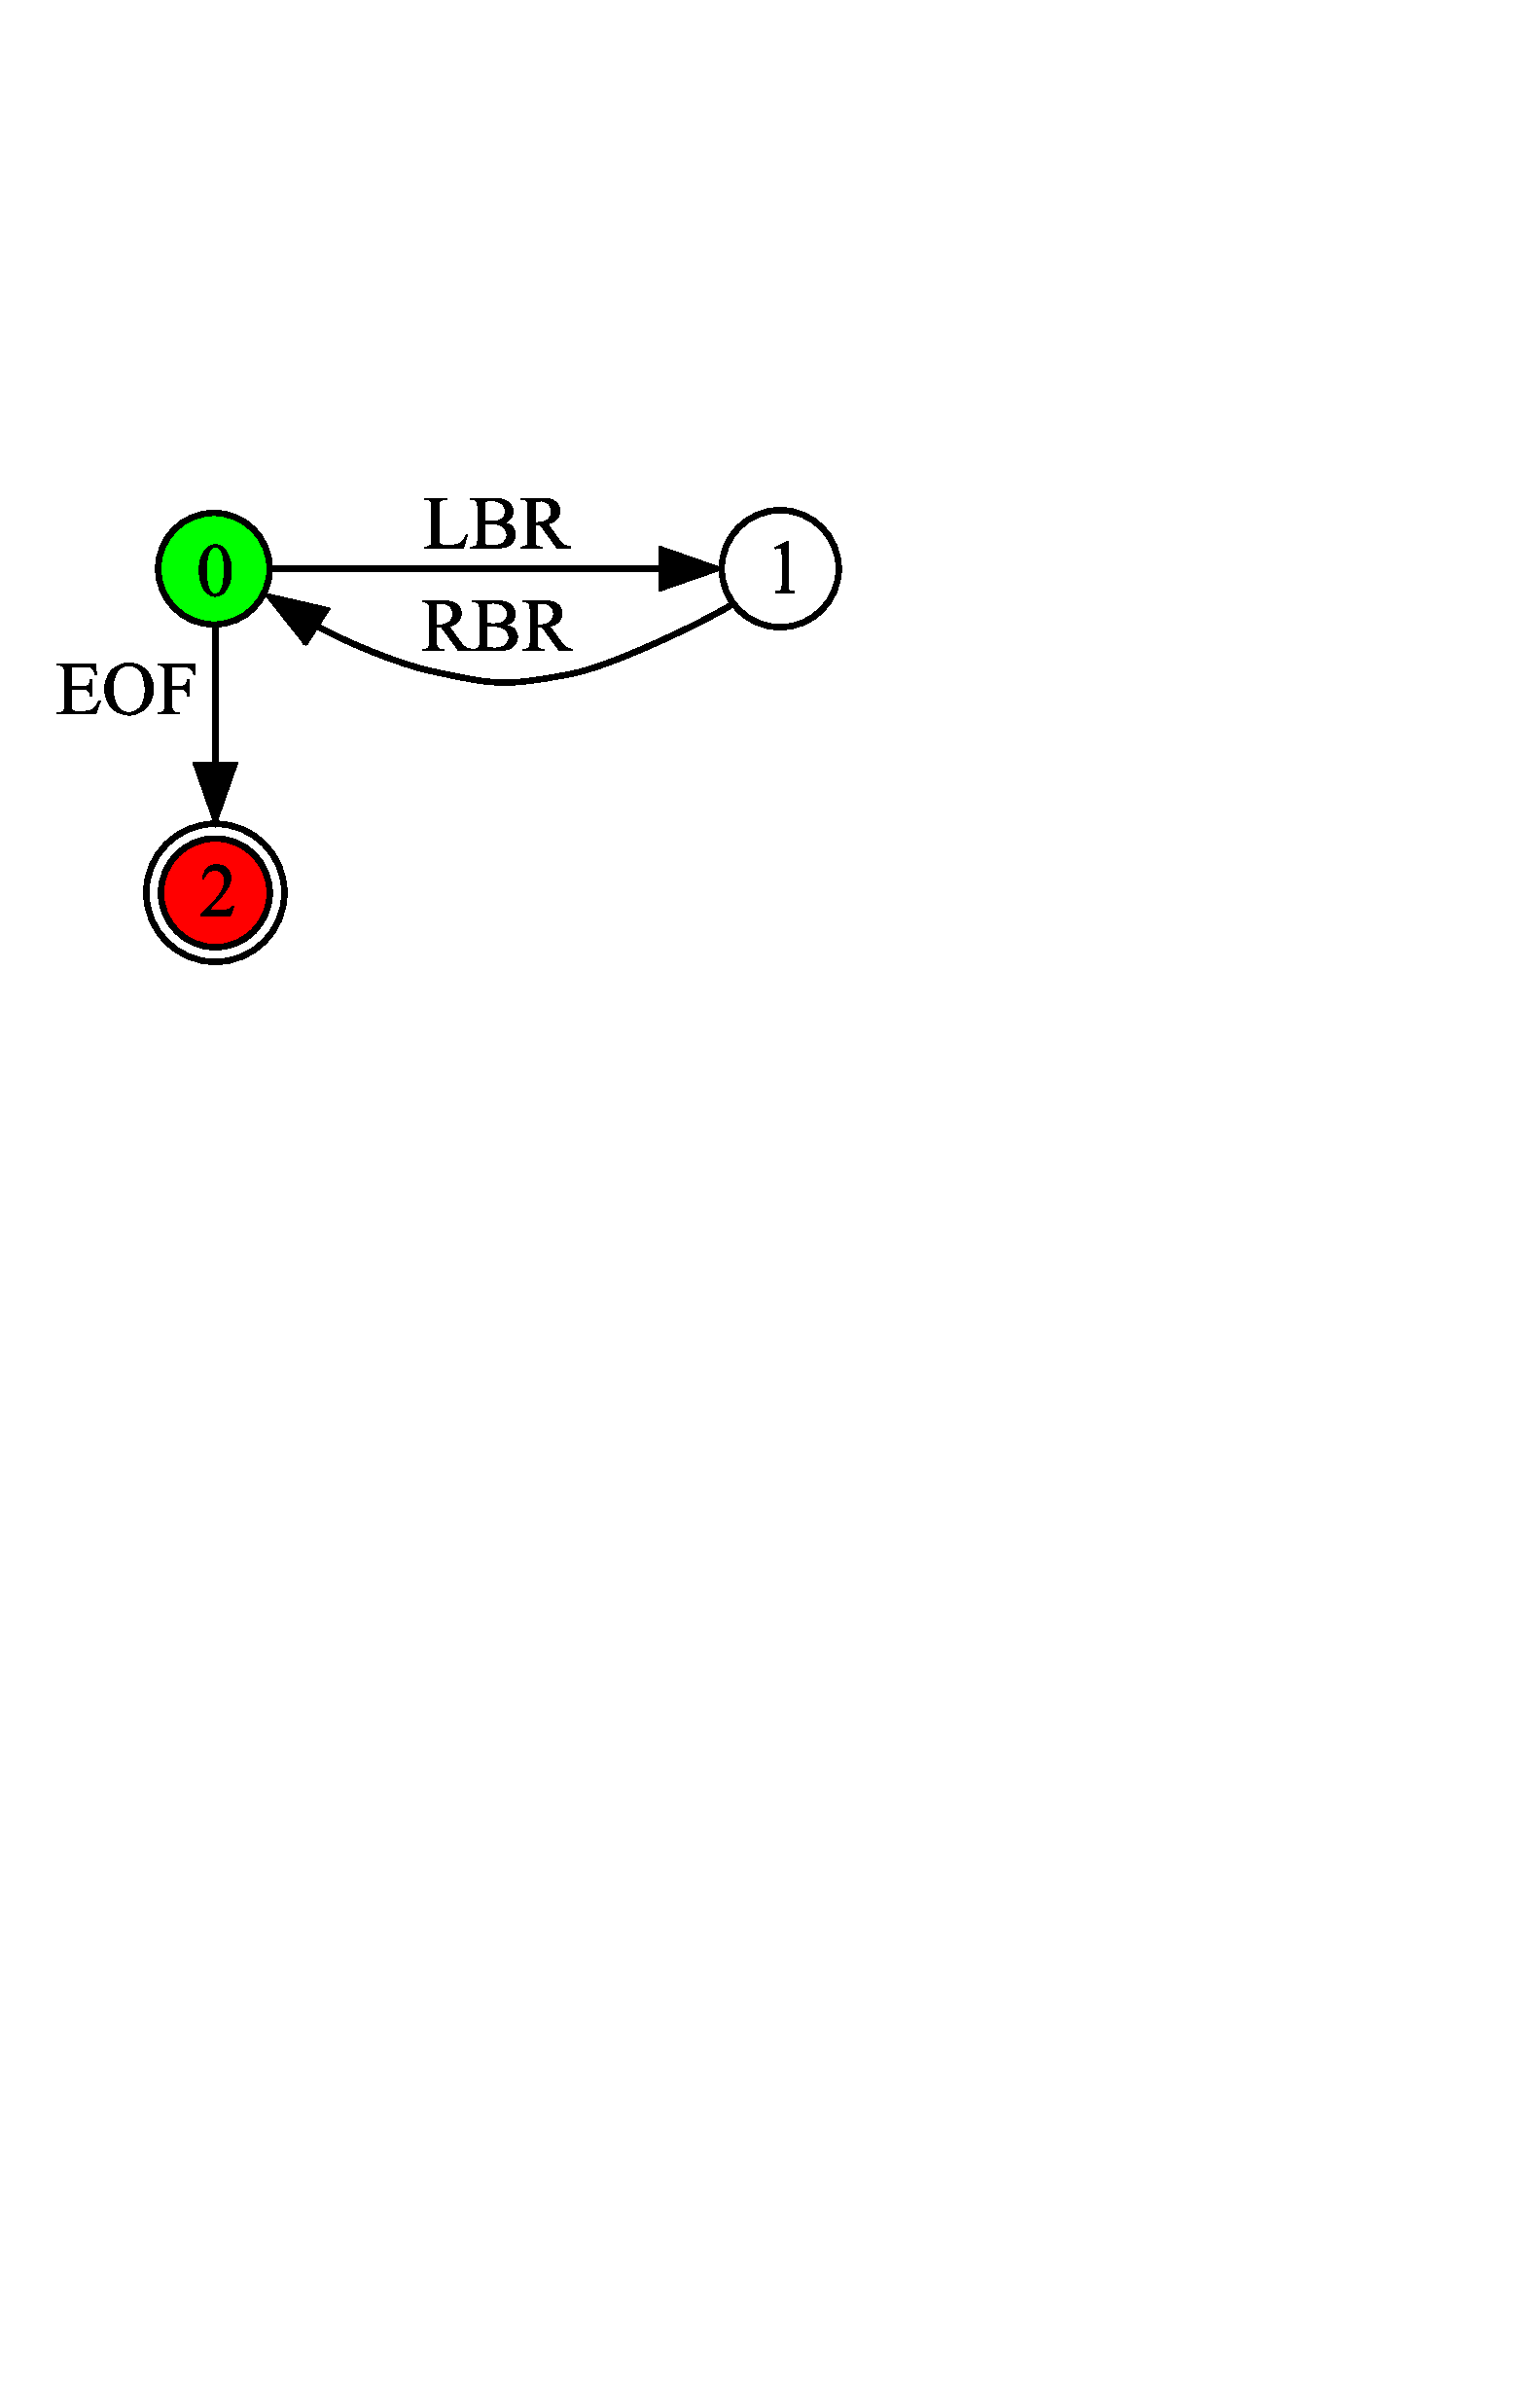
\includegraphics[width=5cm]{pictures/in31.pdf}
&
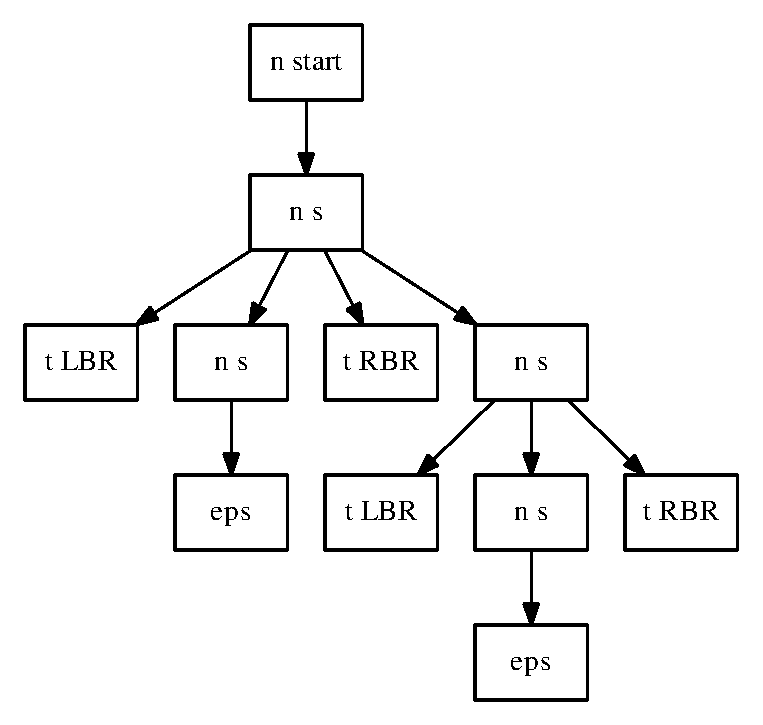
\includegraphics[width=6cm]{pictures/sppf2.eps}
\end{tabular}
\end{frame}


\begin{frame}
  \transwipe[direction=90]
  \frametitle{Algorithm: correctness}
  \begin{theorem}[Termination]
  \normalfont	
    Algorithm terminates for any input
  \end{theorem}
  
  \begin{theorem}[Correctness]
  \normalfont  
    Every tree, generated from SPPF, is correct
  \end{theorem}

  \begin{theorem}[Correctness]
  \normalfont
    For every path $p$ in the inner graph, recognized w.r.t. reference
grammar, a correct tree corresponding to $p$ can be generated from SPPF
  \end{theorem}
\end{frame}

\begin{frame}
  \transwipe[direction=90]
  \frametitle{Implementation}
  \begin{itemize}
    \item The algorithm is implemented as a part of YaccConstructor project 
using F\# programming language
    \item The generator of RNGLR parse tables and data structures for GSS and 
SPPF are reused
 \end{itemize}
\end{frame}

\begin{frame}[t]
  \transwipe[direction=90]
  \frametitle{Evaluation}
  \begin{itemize}
    \item The data is taken from the project of migration from MS-SQL to Oracle Server 
    \item 2,7 lines of code, 2430 queries, 2188 successfully processed
    \item The number of queries which previously could not be processed because 
of timeout is decreased from 45 to 1
  \end{itemize}
  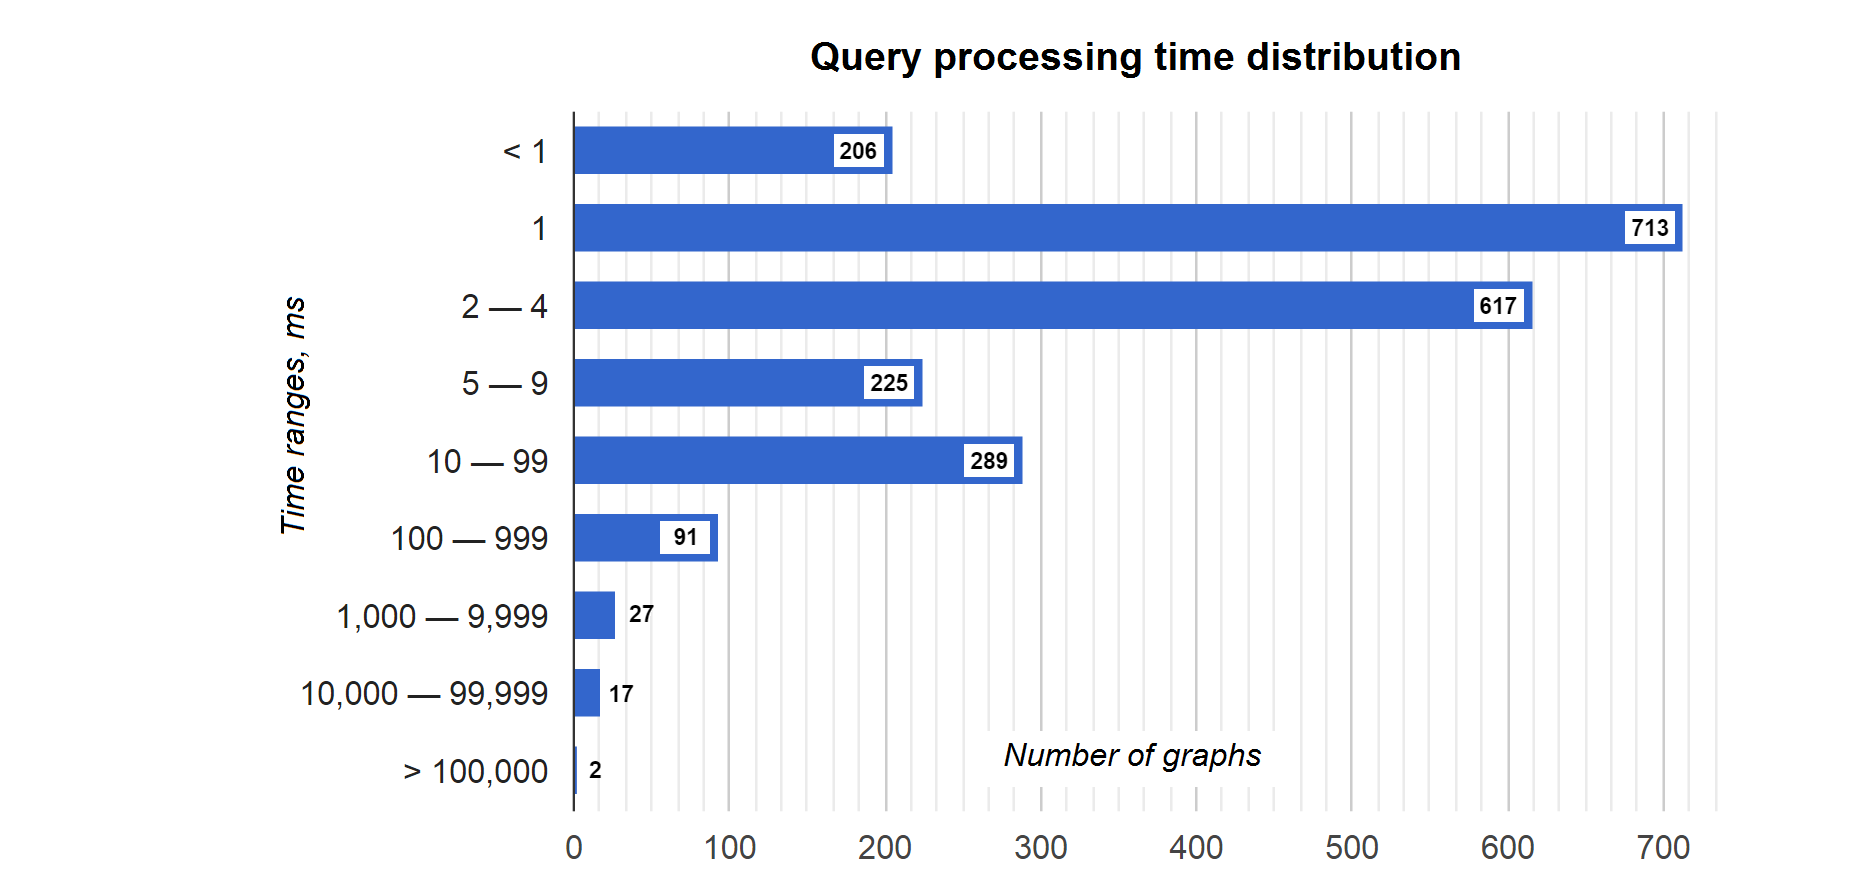
\includegraphics[width=10cm]{pictures/dist.png}
\end{frame}


\begin{frame}
  \transwipe[direction=90]
  \frametitle{Conclusion}
  \begin{itemize}
    \item The algorithm for parsing of regular approximation of dynamically 
generated string which constructs the finite representation of parse forest is 
developped
    \item Its termination and correctness are proved
    \item The algorithm is implemented as a part of YaccConstructor project
    \item The evaluation demonstrated it could be used for complex tasks
  \end{itemize}
\end{frame}

\end{document}
